\chapter{Implementierung des Frameworks}

Dieses Kapitel beschäftigt sich mit der Architektur und Implementierung des Frameworks.
Das Framework schafft eine Abstraktionsebene für die Algorithmen, die die aktiven Topologien in den CEP-Systemen skalieren.
Die reale CEP-Topologie wird in dem Framework als abstrahiertes Graphen-Modell automatisiert erzeugt und den Algorithmen zur Verfügung gestellt.
Dadurch wird ermöglicht, dass Algorithmen, die den Parallelisierungsgrad von Operatoren berechnen, unabhängig vom Zielsystem implementiert werden können.
Anschließend können die implementierten Algorithmen für mehrere verschiedene CEP-Systeme eingesetzt werden, ohne dass Anpassungen am Algorithmus vorgenommen werden müssen.
Außerdem skaliert das Framework automatisch die einzelnen Operatoren mit den berechneten Parallelisierungsgraden.
Die vorliegende Architektur ermöglicht die zeitgleiche Steuerung mehrerer CEP-Topologien, die auch über diverse CEP-Systeme verteilt werden können. 

\section{Architektur}

Die Architektur des Frameworks besteht aus mehreren Komponenten und verfolgt zwei Ziele.
Eines der beiden Hauptziele der Architektur ist, dass das System einfach um weitere Algorithmen erweitert werden kann.
Um dieses Ziel zu erreichen, wurde eine Abstraktionsebene eingeführt, die die Eigenschaften der realen CEP-Topologie repräsentiert.
Diese Abstraktion wird durch ein Graphen-Modell repräsentiert, das einen gerichteten, azyklischen Graphen modelliert.
Die implementierten Algorithmen arbeiten ausschließlich auf dem abstrahierten Modell.
Für die Implementierung eines neuen Algorithmus, müssen nur die Daten aus dem Modell ausgelesen und anschließend verarbeitet werden.
Außerdem ist es möglich mehrere Algorithmen für das gleiche Modell auszuführen und ihre Ergebnisse zu vergleichen.
Um einen Algorithmus für das System zu implementieren ist ausschließlich Wissen über das Modell notwendig.

Ein weiteres Ziel ist, dass das System für weitere CEP-Systeme außer Heron verwendet werden kann.
Dazu wurde eine API, die bereits in einer vorhergehenden Bachelorarbeit entwickelt wurde, erweitert \cite{goggel_vergleich_2018}.
Alle Komponenten des Systems benutzen diese API für die Kommunikation mit dem CEP-System, sodass diese alle system-spezifischen Befehle abstrahieren kann.
Die Seite der API, die mit dem System direkt kommuniziert, ist ein eigenständiger Adapter.
Dieser Adapter wird auf dem Rechner installiert, der das zu steuernde CEP-System kontrolliert.
Der Adapter ist über eine REST-API ansprechbar.
Somit kann das Framework auf einem eigenständigen Rechner installiert werden und das Zielsystem über die REST-Schnittstelle des Adapters kontrollieren.
Dies ermöglicht die Kontrolle von mehreren CEP-Systemen zur gleichen Zeit.
Das Framework kann durch die Implementierung eines entsprechenden Adapters für weitere CEP-Systeme erweitert werden.
Um einen neuen Adapter zu erstellen ist ausschließlich Wissen über die Spezifikation der REST-Schnittstelle notwendig.
Das Framework kann so über die REST-API verschiedene CEP-Systeme über eine einheitlichen Schnittstelle ansprechen.

Die Architektur des Systems ist in der Abbildung 5.1 dargestellt.
Im Folgenden werden die einzelnen Komponenten der Architektur genauer erläutert.

\begin{figure}
  \centering
  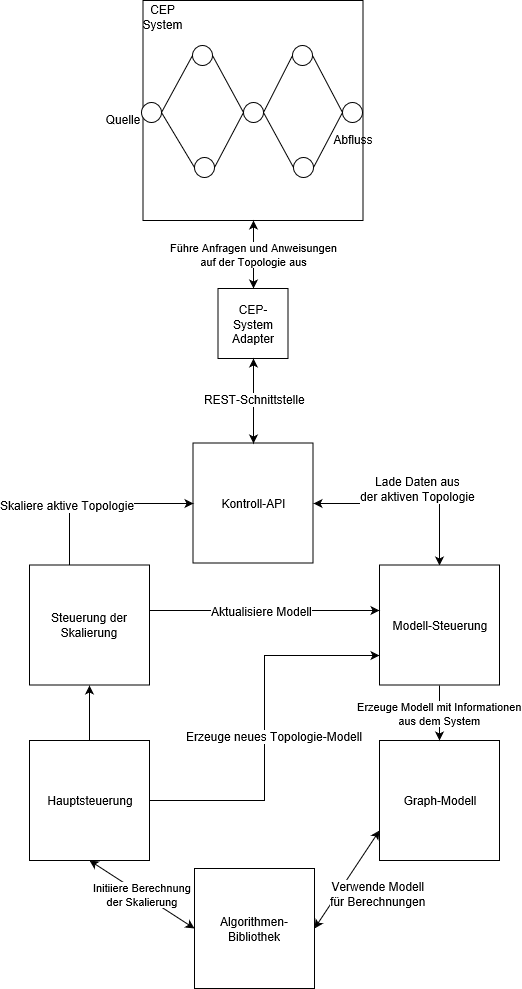
\includegraphics[width=\textwidth]{Systemaufbau.png}
  \caption{Architektur des Frameworks}
  \label{fig:Architektur}
\end{figure}

\section{Graphen-Modell}
Das Graphen-Modell repräsentiert die Topologie im realen CEP-System.
Alle Elemente der Topologie werden nach dem in Kapitel vier vorgestellten Topologie-Modell abgebildet.
Es dient als Cache für Messdaten aus dem realen System.
Durch die Zwischenspeicherung wird ermöglicht, dass ein Modell eines bestimmten Zeitpunktes des realen Systems zur Verfügung gestellt werden kann. 
Würden die Algorithmen die Werte zur Laufzeit abfragen, also immer dann, wenn die Werte benötigt werden, kann dies zu einem inkonsistenten Modell führen.
Die Algorithmen verwenden das Modell, um die Inkosistenz von Messungen zu verschiedenen Zeitpunkten zu verhindern.

Jedes Modell besteht aus Pfaden und Operatoren.
Jeder Pfad stellt dabei eine geordnete Folge von Operatoren dar.
Das Modell erlaubt kreuzende Pfade, sodass Operatoren in mehreren Pfaden verwendet werden können.
Operatoren sind über einen Namen identifizierbar und haben eine dem Parallelisierungsgrad entsprechende Anzahl an Tasks.
Sobald der Operator einen neuen Parallelisierungsgrad erhält, wird die entsprechende Anzahl Tasks gelöscht oder erzeugt.
Somit ist die Anzahl Tasks immer gleich dem Parallelisierungsgrad des Operators.
Der maximale und minimale Parallelisierungsgrad aller Operatoren kann über zwei Konstanten angegeben werden. 
Diese gelten für alle Operatoren in allen Modellen. 
Ein logisch schlüssiger Minimalwert ist ein Parallelisierungsgrad von eins.
Ein Parallelisierungsgrad kleiner als eins ist für einen aktiven Operator nicht gültig, da er keinen ausführenden Task besitzt.
Das Maximum kann entsprechend der Ressourcen, die im CEP-System zur Verfügung stehen, angepasst werden.
Somit kann über Pfade und Operatoren die logische Struktur der Topologie im Modell dargestellt werden.

Die ausführende Ebene, oder physische Struktur, wird durch Tasks und Kanäle repräsentiert.
Tasks sind die Recheninstanzen, die die Operation eines Operators auf Tupel ausführen.
In der vorliegenden Implementierung des Graphen-Modells ist die Zwischenspeicherung der Messwerte auf Task-Ebene vorgesehen.
Somit wird ermöglicht, dass ein detailliertes Modell der Topologie im Frameowork erzeugt werden kann.
Die Kennung der Tasks wird vom Operator automatisch erzeugt.
Sie wird aus dem Namen des Operators und einer fortlaufenden Nummer wie folgt gebildet: \textit{<Name>\_<Nummer>}.
Die niedrigste Nummer ist immer die eins.
Die höchste Nummer entspricht immer dem aktuellen Parallelisierungsgrad des Operators.
Für Tasks sind folgende Messwerte in der aktuellen Version des Modells vorgesehen:

\begin{itemize}
\item{Task-Latenz}
\item{Anzahl Ausführungen des Tasks}
\item{Anzahl eingehender Tupel}
\item{Anzahl ausgehender Tupel}
\item{Auslastung}
\item{Bearbeitungsdauer}
\item{Tupel-Ankunftsintervall}
\item{Varianz der Bearbeitungsdauer}
\item{Varianz des Tupel-Ankunftsintervalls}
\end{itemize}

Wie in Kapitel vier beschrieben wird für die Messwerte der Tasks die Annahme getroffen, dass sie unabhängig vom Pfad sind.
Dies bedeutet zum Beispiel, dass alle eingehenden Tupel durchschnittlich die selbe Bearbeitungsdauer benötigen.
Unabhängig davon von welchem vorhergehenden Operator sie stammen.
Alle für den Task erfassten Metriken differenzieren nicht die Herkunft der Tupel, sondern erfassen sie gesammelt.

Für viele Algorithmen wird nicht der Messwert eines einzelnen Tasks betrachtet, jedoch können die Werte gemittelt beziehungsweise summiert werden um einen aussagekräftigen Messwert für den gesamten Operator zu bekommen.
Um die Messwerte für Operatoren zu berechnen ist pro Messwert eine statische Methode im Modell implementiert.

Die Kommunikation zwischen den Tasks wird durch die Kanäle repräsentiert.
Diese speichern Metriken der Kommunikationskanäle zwischen Tasks.
Für die Implementierung des Modells wurde die Annahme getroffen, dass alle Tasks eines Operators mit allen Tasks der vorhergehenden und nachfolgenden Operatoren kommunizieren können.
Die Anzahl an Kanälen zwischen zwei Operatoren ist also das Produkt aus deren Parallelisierungsgraden.
Für Kanäle sind folgende Messwerte vorgesehen:

\begin{itemize}
\item{Latenz des Kanals}
\item{Latenz der Stapelverarbeitung}
\end{itemize}

Details zu den Messwerten werden in Kapitel 4 erläutert.

\section{Modell-Steuerung}

Die Modell-Steuerung erzeugt die Modellstruktur der Topologien und füllt diese anschließend mit Messwerten.
Alle Aktionen werden von der Hauptsteuerung initiiert.
Im ersten Schritt wird die Topologie vom CEP-System über die Kontroll-API ausgelesen.
Welche Topologie ausgelesen wird entscheidet die angegebene Adapteradresse.
Ein Adapter ist jeweils für eine Topologie zuständig.
Zuerst werden die Pfade der Topologie ausgelesen und im Graphen-Modell die entsprechenden Operatoren und Pfade angelegt.
Dann wird der Parallelisierungsgrad der Operatoren gesetzt.
Wie zuvor beschrieben erzeugen dies durch das Setzen des Parallelisierungsgrades die entsprechende Anzahl an Tasks und Kanälen.
Damit ist das leere Graphen-Modell der Ziel-Topologie erstellt.

Anschließend erzeugt die Modell-Steuerung eine Zuweisung von Tasks im realen System zu den Tasks im Modell.
Die Tasks im Modell sind, wie im vorherigen Kapitel beschrieben, durchnummeriert und haben einen durch das Graphen-Modell festgelegten Namen.
Diese Namen weichen sehr wahrscheinlich von den Namen im realen CEP-System ab.
Damit nun die Messwerte eines realen Tasks konsistent einem modellierten Task zugewiesen werden können, wird pro Operator eine Zuweisungstabelle für die Tasks erzeugt.
Diese Zuweisung muss mit jeder Änderung des Parallelisierungsgrades des Operators angepasst werden, da Tasks wegfallen oder hinzu kommen.
Ist die Zuweisung erfolgt werden zuletzt die Messwerte über die Kontroll-API in das Modell geladen.

\section{Steuerung der Skalierung}

Die Steuerung der Skalierung übernimmt zwei Aufgaben.
Zum Einen werden die Ergebnisse der ausgeführten Algorithmen an das CEP-System geben.
Dazu wird die Kontroll-API verwendet.
Der Adapter passt die Parallelisierungsgrade in der aktiven Topologie an.
Nachdem die reale Topologie erfolgreich angepasst ist wird im zweiten Schritt das Modell angepasst.
Hier werden ebenfalls die neuen Parallelisierungsgrade, die durch den Algorithmus berechnet wurde, gesetzt.
Die Komponente übernimmt somit die Steuerung der Parallelisierungsgrade im Modell und im realen System.

\section{Hauptsteuerung}

Die Hauptsteuerung ist die zentrale Steuereinheit des Frameworks.
Sie enthält die Logik, die die anderen Komponenten kontrolliert und die zuvor beschriebenen Abläufe steuert.
Sie instanziiert die anderen Komponenten für jede Topologie, die gesteuert werden soll.
Außerdem werden die Parameter definiert, die für Berechnungen in den Algorithmen verwendet werden.
Die zeitliche Abfolge aller Abläufe zu steuern ist die Kernaufgabe der Komponente.

\section{Kontroll-API}

Die Kontroll-API abstrahiert die APIs der verschiedenen CEP-Systeme.
Grundsätzlich besteht Sie aus zwei Teilen.
Ein Teil nimmt die Aufrufe aus dem Framework entgegen und wandelt sie in REST-Anfragen um.
Die Anfragen werden anschließend an den entsprechenden Adapter gesendet.
So wird die REST-Schnittstelle über die zur Verfügung gestellten Funktionen gekapselt.
Dieser Teil ist auf der gleichen Maschine wie die anderen Komponenten des Frameworks und wird direkt von den anderen Komponenten angesprochen.

Der zweite Teil, der Adapter, befindet sich auf der Maschine des zu steuernden CEP-Systems.
Er nimmt REST-Anfragen entgegen und setzt diese in Befehle für die API des CEP-Systems um.
Der Adapter ist somit der Teil, der das Kontroll-Schnittstelle des CEP-Systems auf eine einheitliche REST-Schnittstelle abstrahiert.
Außerdem kapselt der Adapter die zurückgelieferten Messwerte des CEP-Systems und vereinheitlicht sie für das Graphen-Modell.
Deshalb ist die Implementierung des Adapters essentiell für die Qualität des Graphen-Modells.
Die Implementierung des Adapters für das CEP-System Heron wird in Kapitel sechs ausführlich behandelt.

Die Kommunikation über die REST-API ermöglicht es, dass die beiden teile auf verschiedenen Maschinen installiert sein können.
Durch die Fern-Steuerung über die Schnittstelle können mit einer einzelnen Installation des Frameworks mehrere CEP-Systeme und Topologien gleichzeitig gesteuert werden.



















